\documentclass[]{tukediphc}
%% -----------------------------------------------------------------
%% tento subor ma kodovanie utf-8
%%
%% na kompilaciu pouzivajte format pdfcslatex 
%%
%% vytvorene distribuciou texlive 2009-7, OS GNU/Linux
%% vytvorene distribuciou TeXLive 2010, OS Win XP
%% februar 2013
%% -----------------------------------------------------------------
\usepackage[utf8]{inputenc}
%\usepackage[T1]{fontenc}
\usepackage{lmodern,textcase}
\usepackage[slovak]{babel}\renewcommand{\figurename}{Obr\'azok}
\def\refname{Zoznam pou\v{z}itej literat\'ury}
\usepackage{latexsym}
\usepackage{dcolumn} % zarovnanie cisiel v tabulke podla des. ciarky
\usepackage{hhline}
\usepackage{amsmath}
\usepackage{nicefrac} % pekne zlomky
\usepackage{upgreek} % napr. $\upmu\mathrm{m}$ pre mikrometer ...
\usepackage[final]{showkeys}%color%notref%notcite%final
\usepackage[slovak,noprefix]{nomencl}
\makeglossary % prikaz na vytvorenie suboru .glo
\usepackage{parskip}% 'zhusti' polozky obsahu
%%
%\usepackage[dvips]{graphicx}
%\DeclareGraphicsExtensions{.eps}
\usepackage[pdftex]{graphicx}
\DeclareGraphicsExtensions{.pdf,.png,.jpg,.mps}
\graphicspath{{figures/}} % priecinok na obrazky
%%
%% Cislovane citovanie
%\usepackage[numbers]{natbib}
%%
%% Citovanie podľa mena autora a roku
\usepackage{natbib} \citestyle{chicago}
% -----------------------------------------------------------------
%% tlač !!!
\usepackage[pdftex,unicode=true,bookmarksnumbered=true,
bookmarksopen=true,pdfmenubar=true,pdfview=Fit,linktocpage=true,
pageanchor=true,bookmarkstype=toc,pdfpagemode=UseOutlines,
pdfstartpage=1]{hyperref}
\hypersetup{%
baseurl={http://www.tuke.sk/sevcovic},
pdfcreator={pdfcsLaTeX},
pdfkeywords={Riadenie procesov, Oceliarstvo, Vizualizácia, Virtuálna realita, Matematické modelovanie},
pdftitle={Elaborát z predmetu Matematické metódy identifikácie, modelovania a simulácie},
pdfauthor={Michal Takáč},
pdfsubject={Dizertačná skúška}
} 
%% nehodiace zakomentujte !
%\dippraca{Elaborát z predmetu Riadenie procesov}
%\bakpraca{Príprava na dizertačnú skúšku}
%%
\nazov{Elaborát z predmetu Matematické metódy identifikácie, modelovania a simulácie}
%% ked praca nema 'podnazov' zakomentujte nasledujuci riadok
%% alebo polozku nechajte prazdnu
\podnazov{}
\autor{Ing.~Michal Takáč}
\veduciprace{prof.~Ing.~Ivo~Petráš, DrSc.}
\univerzita{Technická univerzita v~Košiciach}
\fakulta{Fakulta baníctva, ekológie, riadenia a geotechnológií}
\skratkafakulty{FBERG}
\katedra{Ústav riadenia a informatizácie výrobných procesov}
\skratkakatedry{URIVP}
\odbor{Riadenie procesov}
\specializacia{Kybernetika}
\abstrakt{Abstrakt je povinnou súčasťou každej práce. Je výstižnou
charakteristikou obsahu dokumentu. Nevyjadruje hodnotiace stanovisko
autora. Má byť\/ taký informatívny, ako to povoľuje podstata práce.
Text abstraktu sa píše ako jeden odstavec. Abstrakt neobsahuje odkazy
na samotný text práce. Mal by mať\/ rozsah 250 až 500 slov. Pri
štylizácii sa používajú celé vety, slovesá v činnom rode a tretej
osobe. Používa sa odborná terminológia, menej zvyčajné termíny,
skratky a~symboly sa pri prvom výskyte v texte definujú.}
\klucoveslova{Riadenie procesov, Oceliarstvo, Vizualizácia, Virtuálna realita, Matematické modelovanie}
\datumodovzdania{30. 5. 2020}
\mesto{Košice}

\begin{document}
\renewcommand\theHfigure{\theHsection.\arabic{figure}}
\renewcommand\theHtable{\theHsection.\arabic{table}}
\bibliographystyle{dcu}

\prvastrana


\thispagestyle{empty}
\tableofcontents
\newpage
%
%\thispagestyle{empty}
%%\addcontentsline{toc}{section}{\numberline{}Zoznam obrázkov}
%\listoffigures
%\newpage
%
%\thispagestyle{empty}
%%\addcontentsline{toc}{section}{\numberline{}Zoznam tabuliek}
%\listoftables
%\newpage

%%%%%%%%%%%%%%%%%%%%%%%%%%%%%%%%%

\setcounter{page}{1}
\setcounter{equation}{0}
\setcounter{figure}{0}
\setcounter{table}{0}

\section{Úvod}

%The objective of process control is to keep key process-operating parameters within narrow bounds of the reference value or setpoint. Controllers are used to automate a human function in an effort to control a variable. A basic controller can keep an individual loop on an even point, so long as there is not too much disruption. Complex processes like ones in metallurgy might employ dozens or even hundreds of such controllers, but keeping an~eye on the big picture was, until not so long ago, a human process \cite{Al-Megren2016}.
%
%Cieľom riadenia procesu je udržiavať kľúčové parametre prevádzky procesu v úzkom rozmedzí referenčnej hodnoty alebo požadovanej hodnoty. Ovládače sa používajú na automatizáciu ľudskej funkcie v snahe ovládať premennú. Základný ovládač môže udržiavať jednotlivú slučku na rovnomernom mieste, pokiaľ nedôjde k prílišnému prerušeniu. Komplexné procesy, ako sú procesy v metalurgii, môžu zamestnávať desiatky alebo dokonca stovky takýchto regulátorov, ale pozor na celkový obraz bol až donedávna ľudským procesom \cite{Al-Megren2016}
%
%Although a device was used to automate a human function in an effort to control a variable, there was no sense of what the process was doing overall. A basic controller could keep an individual loop on an even keel, more or less, so long as there was not too much disruption. Complex processes might employ dozens or even hundreds of such controllers, each with its performance displayed on a panel board, but keeping an eye on the big picture was still a human process.	
%
%Aj keď sa zariadenie používalo na automatizáciu ľudskej funkcie v snahe ovládať premennú, nemal zmysel, čo tento proces celkovo robí. Základný ovládač by mohol udržiavať individuálnu slučku na rovnomernom kýli viac alebo menej, pokiaľ nenastane príliš veľa prerušenia. Komplexné procesy môžu využívať desiatky alebo dokonca stovky takýchto kontrolérov, z ktorých každý má svoj výkon zobrazený na doske, ale pozor na celkový obraz bol stále ľudský proces.
%
%The need for developing improved control systems has traditionally been powered by the demand for more accurate and cost efficient production. This is still a major driving force but environmental issues do also have a profound influence on this development today (\cite{Widlund1998}).
%
%Potreba vývoja zdokonalených systémov riadenia bola tradične poháňaná požiadavkou presnejšej a nákladovo efektívnejšej výroby. Je to stále hlavná hnacia sila, ale environmentálne otázky majú na tento vývoj zásadný vplyv aj dnes (\cite{Widlund1998}).
%
%The main objective of controlling oxygen converter steelmaking is to obtain prescribed parameters for the steel when it is tapped from the furnace, including weight, temperature, and each element content. In practical steelmaking process, the criterion whether the molten steel is acceptable or not is often decided by the endpoint carbon content and temperature (\cite{Wang2010}).
%
%Hlavným cieľom riadenia výroby ocele s kyslíkovým konvertorom je získanie predpísaných parametrov pre oceľ, keď sa odoberá z pece, vrátane hmotnosti, teploty a obsahu každého prvku. V praktickom procese výroby ocele sa o konečnom obsahu uhlíka a teplote často rozhoduje o tom, či je roztavená oceľ prijateľná alebo nie \cite{Wang2010}.
%
%Generally, the LD/BOF steelmaking process with sub-lance system can be divided into two stages: static control and dynamic control. Static models include oxygen supplying model, slaging model and bottom blowing model; dynamic models include decarburization speed model, molten steel warming model and the model for the amount of coolant. (\cite{Wang2010}).
%
%The fast dynamics of the LD converter steelmaking process or the BOF process, as it is commonly known, often makes it a challenge to obtain stable blowing conditions and to achieve the required steel composition and temperature simultaneously at the end point. For this reason, process control becomes very necessary and attempts had started as early as in the 1970s (\cite{Fritz2005}). Out of the originally very simple LD process have grown the modern process-controlled and automated production systems that enable present-day adaptations to meet today’s economic and ecological demands (\cite{Sarkar2015}). The non-linear nature of chemical and thermodynamical processes in basic oxygen steelmaking also amassed interest in developing new mathematical models based on fractionalorder calculus.

\section{Matematické metódy}

Parciálne diferenciálne rovnice popisujú fyzikálne procesy pohybu tekutín.

Po špecifikovaní problému, ktorý chceme riešiť, je nutné zostaviť sústavu rovníc popisujúcich problém a zvoliť počiatočné, respektíve okrajové podmienky. Je všeobecne známe, že fyzikálne javy v oblasti dynamiky tekutín

%\begin{figure}[ht!]
%	\centering
%	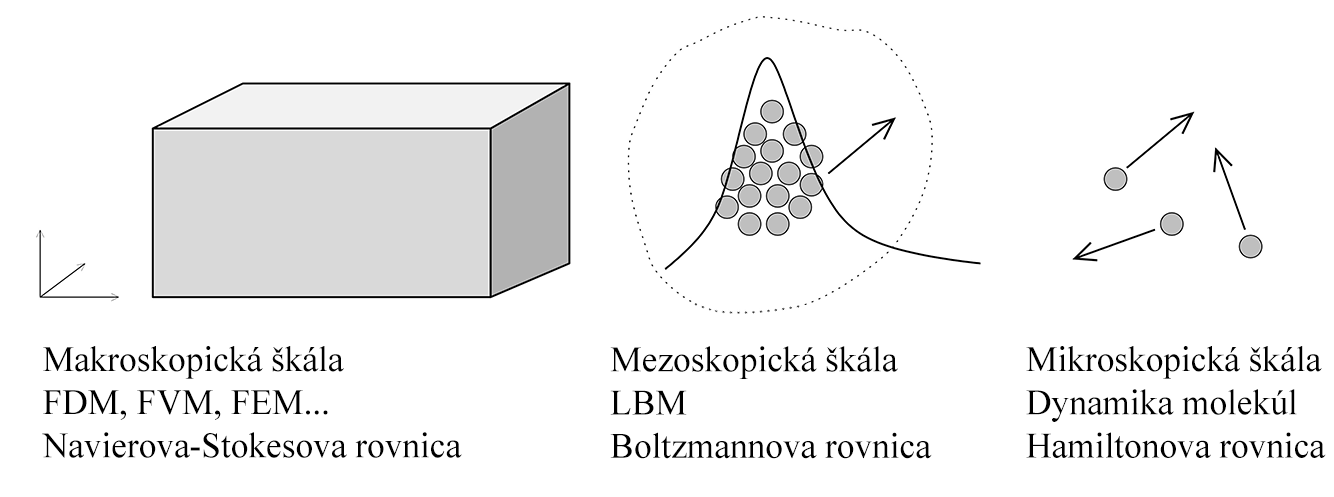
\includegraphics[width=.35\textwidth,angle=0]{figures/different-scales.png}
%	\caption{Rôzne škály.}
%	\label{o:30}
%\end{figure}

\section{CFD analýza}

CFD je využívaná od začiatku 20. storočia v oboroch fyziky akými sú aerodynamika, termodynamika alebo hydrodynamika. Dynamika je časť mechaniky, ktorá sa zaoberá vplyvom pôsobenia síl na pohyb telies.

Aerodynamika sa venuje štúdiom pohybu plynov a ich interakciou s pevnými objektami, akými je napríklad karoséria pretekárskeho auta alebo krídlo lietadla. 

Dynamika kvapalín

Pri skúmaní dynamických javov je cieľom CFD analýzy vytvoriť čo najpresnejší obraz týchto javoch a procesoch, ktoré vznikajú a prebiehajú pri pohybe plynných a kvapalných látok v okolí alebo vo vnútri objektov v pevnom skupenstve. Zároveň je vhodná na analyzovanie toku alebo zmeny teploty v okolí skúmaných objektov. Tieto procesy väčšinou súvisia s pôsobením javov akými sú rozptyl, šírenie, konvekcia, náraz vĺn, klzké povrchy, medzné vrstvy a turbulencia.


% Ukazky z inych odvetvi, relevantnych pre mna?

CFD simulácie sú využívané v rôznych oblastiach, akými sú napríklad prúdenie tekutín v potrubiach, plynov vo vzduchotechnike, analýza chladenia uzavretých priestorov alebo analýzu elektrotechnických zariadení.

Presnosť CFD simulácií ale nie je zaručená a tak treba stále počítať s tým, že nám vedia poskytnúť iba približné informácie o tom, ako sa bude simulovaná súčiastka alebo proces správať v reálnom svete. 


\subsection{Navier-Stokesova rovnica}

Navier-Stokesova rovnica

Jedna zo zaujímavostí je, že Clayov inštitút vypísal na nájdenie riešenia Navier-Stokesovej rovnice odmenu 1 milión dolárov. 

\subsection{Metóda lattice Boltzmann}

Metóda lattice Boltzmann je relatívne nová metóda v oblasti CFD analýzy.

\subsection{LES}

\subsection{DNS}

\section{Počítačom podporované matematické modelovanie}

Počítačom podporované inžinierstvo (CAE - Computer Aided Engineering) je použitie počítačového softvéru na simuláciu výkonu s cieľom vylepšiť návrhy výrobkov alebo pomôcť pri riešení technických problémov pre celý rad priemyselných odvetví. To zahŕňa simuláciu, validáciu a optimalizáciu produktov, procesov a výrobných nástrojov.

Typický proces CAE pozostáva z krokov predbežného spracovania, riešenia a následného spracovania. Vo fáze predspracovania inžinieri modelujú geometriu (alebo reprezentáciu systému) a fyzikálne vlastnosti návrhu, ako aj prostredie vo forme aplikovaného zaťaženia alebo obmedzení. Ďalej je model vyriešený pomocou vhodnej matematickej formulácie základnej fyziky. Vo fáze po spracovaní sa výsledky predložia technikovi na preskúmanie.

Aplikácie CAE, výhody používania CAE...

\url{https://www.plm.automation.siemens.com/global/en/our-story/glossary/computer-aided-engineering-cae/13112}

Motivácia na používanie počítačových simulácií na skúmanie metalurgických procesov je dvojaká. Po prvé, umožňuje testovať zmeny dizajnu pred vytvorením prototypu, čo samozrejme vedie k nižším celkovým nákladom na návrh. Po druhé, umožňuje skúmať javy, ktoré sa nedajú ľahko merať alebo pozorovať v procese. Dokonca aj zdanlivo jednoduchá operácia, ako napríklad nepretržité meranie teploty počas procesu oduhličovania, je zložitá z dôvodu veľmi vysokých teplôt v procese a všeobecne drsných podmienok prevládajúcich v oceliarňach (\citep{Ersson2018}).

V metalurgii pri výrobe ocele je veľmi dôležité simulovať lineárne a nelineárne procesy, s ktorými sa pri výrobe ocele stretávame pri tvorbe matematických modelov. Od prvých pokusov o využitie matematických techník na simuláciu a optimalizáciu veľkých metalurgických operácií (Ray a kol., 1973) sa zaviedli rôzne numerické metódy ako algoritmy a použili sa na simuláciu javov v oceliarskych procesoch. Jednou z tried takýchto metód je Monte Carlo, ktoré je užitočné na simuláciu systémov s mnohými stupňami slobody, ako sú tekutiny.
Problémy s modernou mechanikou tekutín by nebolo možné vyriešiť bez použitia výpočtovej dynamiky tekutín (CFD), pretože rozsah analytických riešení základných rovníc mechaniky tekutín je veľmi obmedzený a keď sa dosiahne zložitejšia geometria, zvyčajne na výber riešenia musia zvoliť danú numerickú metódu. CFD zahŕňa široké spektrum numerických metód používaných pri riešení komplexné trojrozmerné (3D) a časovo závislé problémy s tokom (\citep{RAPP20173}). Od počiatku priekopníckej práce v oblasti metalurgie, ktorú uskutočnili Szekely a kol. (1977), náklady na vykonávanie počítačových simulácií sa za posledných niekoľko desaťročí znížili, zatiaľ čo dostupný spracovateľský výkon sa zvýšil. Väčšina procesorov a spracovateľských jednotiek, ktoré sa v súčasnosti vyvíjajú a vyrábajú, má niekoľko jadier, ktoré môžu vykonávať pokyny súbežne. Spracovateľský výkon, ktorý je k dispozícii pre softvér CFD, teda tiež závisí od schopnosti softvéru vykonávať paralelne. Štúdia z posledných dvoch desaťročí (\citep{Ersson2018}) simulácií metalurgického CFD odhaľuje obrovské zlepšenia týkajúce sa typu javov, ktoré je možné preskúmať, a tento trend bude pokračovať vďaka zlepšeniam v dostupnom spracovaní. výkon a dostupné algoritmy. Preto CFD našiel cestu do mnohých štúdií v oceliarstve, kde sa tieto metódy ukázali ako užitočné pri preukazovaní skrytých a významných vlastností. Jeho použitie v oceliarskom priemysle však nemusí byť také integrované ako v leteckom a automobilovom priemysle, v ktorých je vývoj nových dizajnov kľúčový. Hlavný rozdiel medzi leteckým a metalurgickým priemyslom spočíva v tom, že hutnícky priemysel sa takmer vždy zaoberá viacfázovými systémami pri zvýšených teplotách a že motiváciou modelovania je najmä optimalizácia procesov. S pokračujúcim vývojom vo viacfázových modeloch, ako aj pri reakčnom modelovaní toku, ostáva pokračujúca užitočnosť CFD v metalurgii jasná.

V procese LD / BOF určujú rôzne chemické reakcie medzi kyslíkom, troskou a roztaveným železom v konvertore kyslíka, v kombinácii s energickým miešaním, aby sa podporila troska, defosforizácia, dekarbonizácia, zahrievanie roztavenej ocele a homogenizácia zloženia a teploty ocele. výsledné vlastnosti ocele. Cieľom konvertora kyslíka je rafinovať roztavené železo na surovú oceľ oxidáciou, aby sa dosiahla konečná teplota a chemické zloženie na konci rany. Ak to neurobíte, bude to potrebné zrevidovať. Vplyv prúdu kyslíka do roztaveného kúpeľa silne ovplyvňuje kúpeľ a podporuje trojfázový tok medzi plynom, troskou a roztavenou oceľou v kúpeli. S prechodom od starých systémov založených na pravidlách k modelu v reálnom čase uzavretým

\subsection{Computational Fluid Dynamics}

\subsection{Programy pre CFD simulácie}

Matlab

Ansys

SimScale

OpenFOAM

%
%%
\Urlmuskip=0mu plus 1mu\relax
\bibliographystyle{spbasic}
\bibliography{refs/control,refs/mathematics,refs/modeling,refs/cfd,refs/lbm,refs/gpu,refs/interaction,refs/interfaces,refs/hci,refs/design,refs/ml,refs/visualization,refs/programming,refs/simulation,refs/ar,refs/vr,refs/online}

%

\end{document}
%%